%
\section{Calculation of coda q, CODAQ}

\index{Quality factor}
\index{CODAQ} 
This section contains the main program CODAQ to calculate coda Q, program CODAQ\_AREA to sort output from CODAQ into areal bins and a help program AVQ to average Q-relations.

Codaq

The program will calculate coda Q (hereafter called Q) for a series of events and stations at given frequencies. On completion, the average values are calculated and a Q vs f curve is fitted to the calculated values. The program will also plot the individual events and filtered coda windows. 

The principle for calculation is the standard coda Q method, whereby a coda window is bandpass filtered, an envelope fitted and the coda Q at the corresponding frequency calculated. The envelope is calculated RMS value of the filtered signal using a 5 cycle window. The program used here is the one described in \citet{havskov1989}. \index{Quality factor, determine with coda}
%�\textcolor{red}{jh-comment: next section rewritten, pelase check...}
The program can only operate in connection with the SEISAN format S-files. The program can use all waveform file types accepted by SEISAN and there can be more than one waveform file in the S-file.  The program will also take advantage of the SEISAN database structure.  

Input: \newline
The calculations are controlled by a parameter file called co\index{Codaq.par}daq.par and the actual event-station combinations to use are given in \index{Codaq.inp}\texttt{codaq.inp}. Example files are in DAT, and with the test data set and the example files in DAT, a test run can be done. An example of a parameter file is shown below: 

\verbatiminput{include/codaq.par}

Start in s-times and Vp/Vs ratio (optinal): Normally the coda window starts at twice the S-travel time from the origin, this factor can be varied and might be chosen differently in special cases. Note that the S-time is calculated from the P-time so a P-time must be present. This also means that if a Pn is used, the coda window will start at 2 times the Sn travel time, which might be substantially different from 2 times the Sg travel time. 
%\textcolor{red}{jh-change: Th
e S-time is calcualted from the P-time using and Vp/Vs = 1.78. 
Optionally, the user can select an Vp/Vs ratio to be used. 
This parmeter is optional so parameter files prior to version 8.3 can be used. 

Absolute start time: If 0.0, above parameter is used. However if different from zero, an absolute start time relative to the origin time is used for the start of the coda window. This might be useful since different start times (meaning different lapse times) might produce different q-values. To use this parameter, one must be certain to choose it long enough which can be checked with the plots. If the absolute start time is smaller than (Start in s-times) multiplied by the s travel time, the station will be skipped and a message given. 

Window length: This is the coda window length in secs. Use at least 20 secs to get stable results. 

Spreading parameter: The geometrical spreading parameter used in q-fit, normally 1.0 is used. 

Constant $v$ in $q = q0*f**v$ : For all $q(f)$ values, $q0$ is calculated using a fixed $v$, use e.g. $1.0$. This parameter has no influence on the individual $q$ calculations. 

Minimum signal to noise ratio: In order to accept a q value for the average, the signal to noise ratio must be above this value. The signal to noise ratio is calculated using the last tRMS ( see next parameters) secs of the filtered coda window and the first tRMS secs of the data file window. If the data file starts with noise or in the P signal, the s/n ratio will be in error. A reasonable value is 5.0. 

Maximum counts to use: If the count value in a coda window is above this value, the window is not used. The intention is to avoid using clipped values. From SEISAN version 7.2, there is also an automatic checking for clipped values in addition to `maximum counts'. 

Noise window in front of signal and length of noise window, tnoise and tRMS: The first number is the number of seconds of noise to plot in front of the signal. In previous versions, 15 secs was hardwired, but sometimes there was not 15 secs of noise before the P. The second number is the length of the noise window used for calculation of the signal to noise ratio. This was earlier hardwired to 5 secs. 

Minimum correlation coefficient: In order to use the q value in the average, the correlation coefficient of the coda q fit must be larger than or equal to this value. NOTE. Correlation values are in reality negative, but are always referred to as positive in the following. An acceptable value depends on the data, try to use a value higher than 0.5 (in reality -0.5) 

Number of frequencies: Number of frequencies to use, maximum 10, 5 is a good number. 

Frequencies and bands: The corresponding center frequencies and frequency 
bands. The frequency band should increase with increasing frequency 
to avoid ringing. E.g. 8,3 means that the signal is filtered between 
6.5 and 9.5 Hz. It is advisable to use constant relative bandwidth 
filtering, to get an equal amount of energy into each band. The relative 
bandwidth is defined as $RBW = ( f_u - f_l )/ f_o$ where $f_u$ and $f_l$ are 
upper and lower frequency limit respectively. Such a filter would 
be e.g. $4\pm1$, $8\pm2$. $16\pm4$. The frequency representing the energy in a 
particular filter band, is the geometric center frequency calculated 
as $f_c = sqrt{f_u f_l }$.
Since the user probably wants to calculate coda Q at the given frequency, the normal 
option (new in SEISAN7.2) is that $f_u$ and $f_l$ are calculated such that the 
given bandwidth (e.g. 4 Hz) is used, but the actual $f_u$ and $f_l$  will 
give the specified central frequency. It is still possible to calculate 
as before, where $f_u$ and $f_l$  will be exactly as specified (but the 
geometrical center frequency will not correspond to specified center 
frequency) by giving the bandwidth as a negative number. 

Default stations: The stations that will be used if not specified in the \texttt{codaq.inp} file. THE LINE MUST CONTAIN AT LEAST SOME BLANK CHARACTERS, if not, stations will not be read from \texttt{codaq.inp} file and the program will crash. Note also that the program will use the first available component in waveform file if no components given in the line following. After reading the parameter file, the program will by default use the \texttt{codaq.inp} file to get the event station information. However, any other name can be used if specified interactively, see below. The station codes can have up to 5 characters. 

The \texttt{codaq.inp} file will consist of a series of lines each giving an event identifier (an INDEX file).  An easy way to generate the file is using the SELECT program. The file can also be generated with EEV using the (C)opy option making a file called indexe\index{Indexeev.out}ev.out. An example is shown below: 

\begin{verbatim}
    1  /top/seismo/seismo/REA/BER__/1992/06/16-0343-38L.S199206
    3  /top/seismo/seismo/REA/BER__/1992/06/16-1311-58L.S199206
    7  /top/seismo/seismo/REA/BER__/1992/06/30-1504-30L.S199206 
\end{verbatim}

The above example only uses the default stations given in \texttt{codaq.par}. Below is an example where particular stations and components have been selected with particular events, for this to work the station line in \texttt{codaq.par} MUST be blank. 

\begin{verbatim}
    1 /top/seismo/seismo/REA/BER__/1992/06/16-0343-38L.S199206
HYA  KMY  BER  ASK  TRO
S  Z S  E B  E S  Z S  Z 
    3 /top/seismo/seismo/REA/BER__/1992/06/16-1311-58L.S199206
HYA 
    7 /top/seismo/seismo/REA/BER__/1992/06/30-1504-30L.S199206
HYA  EGD
S  E  S  Z 
\end{verbatim}

Note that the numbers to the left originate from the index file and do not have any importance. The long name with the directory structure, is the name of the pick file (S-file) in the database, if the S-file is in the local directory, it can have just the event id, in this example starting with 30-....The waveform file name is in the S-file. Following the S-file name is, (like in the parameter file), first a line with station codes followed by a line of component codes. Like in the parameter file, if a component is not given, it will be assumed that the component is S Z. THE COMPONENT LINE MUST BE THERE, EVEN IF BLANK. Since it can be quite a lot of work to generate this file manually with both stations and components, SELECT has an option to generate it, see SELECT. However, SELECT will not give component names so only one componet is used (the first in the waveform file). The file from SELECT is called index.codaq. 
/index{index.codaq}

Below is an example of a \texttt{codaq.inp} file, where it is assumed that the S-files are the current directory. This file can also be generated with DIRF. 

\begin{boxedverbatim}
       16-0343-38L.S199206
HYA  KMY  BER  ASK  TRO 

       16-1311-58L.S199206
HYA
S  E 
       30-1504-30L.S199206
HYA  EGD
S  N S  E 
\end{boxedverbatim}

Program operation: \newline
The program first reads the parameter file, default \texttt{codaq.par} which must be in your current directory. It then reads the \texttt{codaq.inp} file with the events to analyze (also in current directory). The S-file names given here can, as shown in the examples above, be in the database or elsewhere, e.g. in your local directory. In the S-file, the name of the waveform file is given. If more than one waveform file is given, all files will be searched for the specified station and component. The program will first look in the current directory, and then in WAV and thereafter in the WAV database and other directories as given in the \texttt{SEISAN.DEF} file in DAT. The program can therefore work without moving the data from the database, however you can also move both the S- files and waveform files to your local directory. Remember that the S-files must be updated in order to have origin time, since the program uses the origin time and P arrival times from the S-files. 

Running the program: 

\verbatiminput{include/codaq.run}

The program will now start to run. 
%\textcolor{red}{jh-change: 
Alterantively, the progran can be started 
with arguments on the promt line:

\texttt{codaq n parameter-file data-file}

and no questions are asked. n is the choice 0 to 3 above.

If no plot is chosen, one line will appear on the screen for each station used and one for each frequency. The program will start a new page for each new event. If you are plotting on the screen, you will therefore have to hit return to get the next plot. The screen might not have been filled out if there are few data. 

All questions will appear in the text window. At the end, a summary is given, which is the same as logged in the output file \texttt{codaq.out}. 

The abbreviations are: 

\begin{tabular}{lp{10cm}}
H: & Focal depth \\
M: & Magnitude \\
TP: & P travel time \\
TC: & Start time of coda window relative to origin time \\
F: & Frequency \\
Q: & Corresponding coda q, if 0 value is $>$ 10000 or negative \\
S/N: & Signal to noise ratio AV \\
Q: & Average q \\
SD: & Standard deviation for average \\
NT: & Total number of q values at all frequencies \\
N: & Number of q values at given frequency \\
q: & Average of q values \\
1/q: & q is calculated as 1/q  averages, probably the best to use \\
f:1/q: & Q values calculated using the relation derived from the 1/q averages \newline
q = q0*f**v obtained with the average 1/q-values \\
cq0: & Constant q0 obtained using the fixed user selected v \\
v: & Constant v determined \\
%\textcolor{red}{jh-change:} 
cor: & Correlation coefficient on determining q vs f \\
%\textcolor{red}{jh-change:} 
corr: & Average correlation coefficients of individual 
codaq calculations when fitting the envelope, both average and standard deviation is given \\
\end{tabular}

If a station is not present or no P is read, a message will be given. The program will search for the first P arrival time in the S-file. If several are present for the same station, it will use the first. 

Output: 

A file called \texttt{codaq.out} is generated. It contains a copy 
of the parameter file, one line for each event station combination 
accepted by the program (correlation and s/n ratio) and the average 
$q$ values. The $q$ values are averaged directly (indicated by $q$) and $1/q$ 
are averaged (indicated by $1/q$). At the end are the fits to the $q = q0*f**v$ relation. A summary of codaq.out is given in codaq1.out 
%\textcolor{red}{jh-change: 
This relation is calulated using the average Q-values for each frequency and each average is weighted by the number of observations used to calculate the average.  

Output of codaq midpoints, codaq.area

For each accepted Q value, the midpoint between the station and the event together with the corresponding Q and frequency is saved in the file, see example below

2009 1 2 03134 RTCT  -32.25 -67.39    8.0  612.0
2009 1 3 452 6 CFAA  -31.67 -68.16   12.0  881.0
2009 113101828 SALAG -32.63 -68.77   12.0  740.7
2009 118 3 521 RTLL  -31.22 -68.50    1.0  310.1
2009 126185753 AGREL -33.15 -68.95    1.0   61.9

The content is: Event date, station code, lat -lon of midpoint, frequency and Q. This information can be used to plot the areal variation in Q and SEISAN provides one such program, CODAQ\_AREA, see below.

%\textcolor{red}{jh-change:
A file called \texttt{codaq.index} is created. This index file contains all the events accepted for calculating the codaq values and can therefore e.g. be used for making an epicenter map of events actually used (use collect with the index file)  
Output file \texttt{codaq1.out} contains the same output as \texttt{codaq.out} except there is no \texttt{print out} for each event. 

Example of \texttt{codaq.out}: 

\verbatiminput{include/codaq.out}

Above, the one line per q calculations is showing results from different stations. Only the traces selected (fulfilling selection criteria) are shown. The time indicated, is the start time in the waveform file for that particular station. 
In general, the start time for each channel of digital data would be different. If some data is missing, it is also show in the \texttt{codaq.out} file. Corr is the average correlation coefficient (with standard deviation) for the data selected for that frequency. The average lapse time is the average of the tc - values. 

In the DAT directory, there is an example \texttt{codaq.par} and \texttt{codaq.inp} set up to run on PC assuming that SEISAN has been installed under \\seismo. If installed differently, edit the \texttt{codaq.inp} file to reflect the installation. For Unix testing, the \texttt{codaq.inp} MUST be edited to reflect the installation path or the file is regenerated using EEV as described above. 

General recommendations: Coda window should be 15-25 seconds, minimum correlation coefficient larger than 0.5. For comparing coda values in different regions, ALL processing parameters must be identical and average lapse times should be very similar. 

Figure \ref{fig:codaQ} gives an example of a codaq plot. There are 
no options for the codaq plots and the length of the window is always 
the first 200 secs from the original trace. If origin time or coda 
window is outside this 200-sec window and data is available, the 
program continues, but the coda window is not plotted on the figure. 

\begin{figure}
\htmlimage{scale=2.0}
\centerline{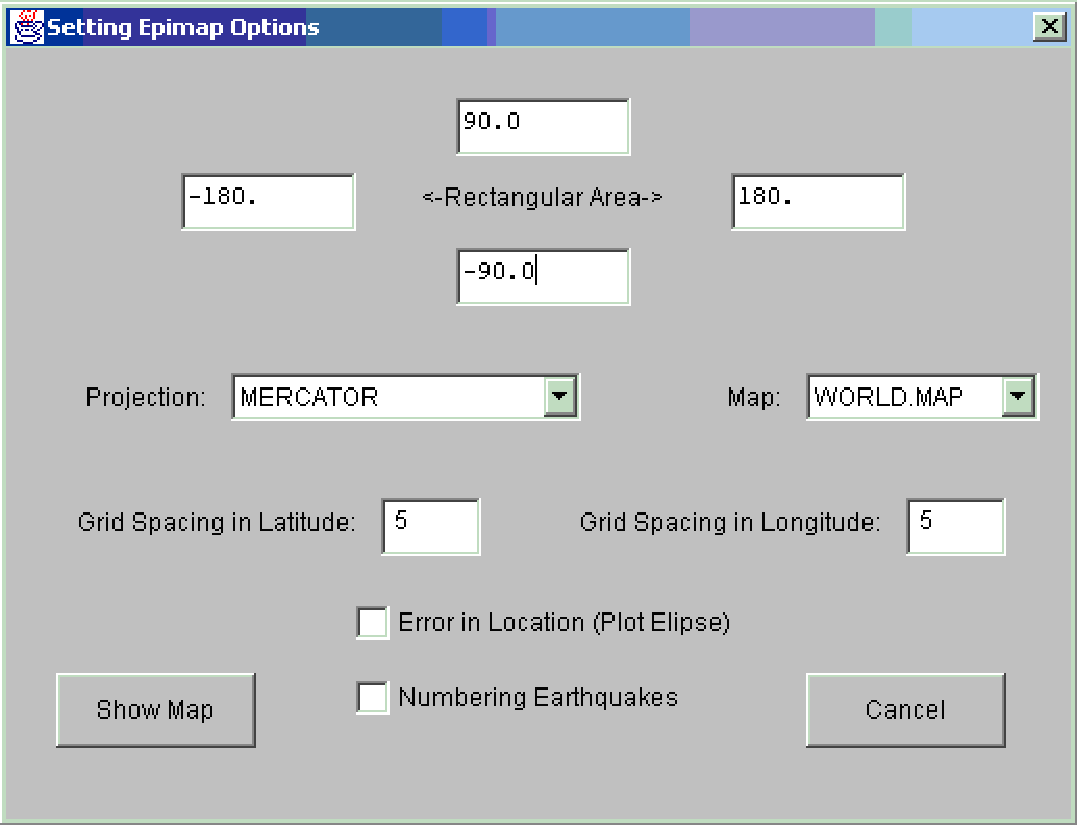
\includegraphics[width=0.9\linewidth]{fig2/fig8}}
\caption{
An example of a coda Q plot. On top is shown the original 
trace and below the filtered coda windows. Note that 15 secs of noise 
are shown in front of the selected filtered coda window. The first 
5 secs of the noise shown is used for calculating the S/N ratio. 
On each filtered plot is given F: Center frequency, Q: Q-value, zero 
means no Q-value could be calculated, S/N: Signal to noise ratio. 
}
\label{fig:codaQ}
\end{figure}


Program CODAQ\_AREA
\index{CODAQ\_AREA}

CODAQ outputs the Q-values at midpoints between station and events. CODAQ\_AREA reads this output and, at each frequency, average Q-values in user defined lat-lon bins. In each bin, provided there is enough data, the Q relation  $q = q0*f**v$  is also calculated. The values in each bin is listed in an output file which can be displayed to get an approximate idea of the areal Q-distribution.

Input files:
It is assumed that codaq.area exists so this name is hardwired. The corresponding codaq1.out is also used to get the frequencies used. 

The interactive options are:

Min no for grid average, min no of freq for Q0 calculation:
Minimum number of Q-values in a bin in order to do an average for that bin, minimum number of frequencies for which Q was calculated in a particular bin in order to calculate Q-relation.

Latitude range and grid size:
Longitude range and grid size: 
Range to use and size of grid in degrees, can be a fraction of a degree.

The interactive options can be stored in a file called codaq\_area.inp. If the file is present, input will be read from that file and no questions asked.

Example run:

\begin{verbatim}
C:\>codaq\_area
Frequencies    1.00    2.00    4.00    8.00   12.00   16.00
 Min no for grid average, min no of freq for Q0 calculation
3 4
 Lattitude range and grid size
-34 -28 1
 Longitude range and grid size
-71 -66 1
 Number of q-data in input file        1094
 Number of q-data inside grid           560


 File with areagrid:    codaq_area.out
 File with grid points: codaq_grid.out
\end{verbatim}

Part of areal output file coda\_area.out showing the lat-lon bins, note the midpoint of the bin is used:

\begin{verbatim}
freq=   1.0000000    
       -70.5 -69.5 -68.5 -67.5 -66.5
 -28.5     0     0     0    49    48
 -29.5     0     0    88     0     0
 -30.5     0     0    42     0     0
 -31.5     0     0    61     0     0
 -32.5     0    57    55     0     0
 -33.5     0     0    67     0     0
 freq=   2.0000000    
       -70.5 -69.5 -68.5 -67.5 -66.5
 -28.5     0     0     0   120   117
 -29.5     0     0   115     0     0
 -30.5     0     0   131     0     0
 -31.5     0     0   111     0     0
 -32.5     0   110   145     0     0
 -33.5     0     0     0     0     0
\end{verbatim}

Output file codaq\_grid.out contains details of the averages in each bin see part of file below:


\begin{verbatim}
freq=   1.0000000
   -33.500   -70.500       0.0       0.0         0
   -33.500   -69.500       0.0       0.0         1
   -33.500   -68.500      67.1      20.6         8
   -33.500   -67.500       0.0       0.0         0
   -33.500   -66.500       0.0       0.0         0
\end{verbatim}

The output is: Bin midpoint, average Q, standard deviation in average and number of points in bin.



Program AVQ, average Q-relations

Q as a function of frequency is usually described as

 $q = q0*f**v$ 

If several such relations are to be averaged, it is not just a question of averaging the parameters. In program AVQ, the averaging is done in the following way:

-For each relation, 1/Q is calculated at the frequencies 1, 2, 4, 8 and 16 Hz.
-At each frequency, average 1/Q is calculated using the number of observations in the original determination of Q for a particular relation as weight.
-A new least squares determination of  $v$ in $q0$ is made with the Q-values.

The program uses an input file with q0, v and number of observations, one relation (free format) per line. An example of a run is seen below:

\begin{verbatim}
C:\seismo\WOR>avq
 File name
input.txt
 Q0,alpha,n   100.00000      0.50000000            1000
 Q0,alpha,n   200.00000       1.0000000              10
 Q0,alpha,n   150.00000      0.69999999             500
  Number of curves to average:            3
  Total number of observations        1510
 Q0,alpha,corr   113.20638      0.54150712      0.99998659
\end{verbatim}


/index{AVQ}
/index{Average Q-relations}



